\documentclass[problem]{mcs}

\newcommand{\neutr}{\ensuremath{\mathbf{N}}}

\begin{pcomments}
  \pcomment{MQ_3color_XOR}
  \pcomment{variant of CP_3color_OR_gate, PS_3color_SAT}
  \pcomment{ARM Mar 22, 2014; revised 4/7/15}
\end{pcomments}

\pkeywords{
coloring
xor
}

%%%%%%%%%%%%%%%%%%%%%%%%%%%%%%%%%%%%%%%%%%%%%%%%%%%%%%%%%%%%%%%%%%%%%
% Problem starts here
%%%%%%%%%%%%%%%%%%%%%%%%%%%%%%%%%%%%%%%%%%%%%%%%%%%%%%%%%%%%%%%%%%%%%
\begin{problem}
In the graph shown in Figure~\ref{fig:3color-XOR}, the vertices
connected in the triangle on the left are called
\emph{color-vertices}; since they form a triangle, they are forced to
have different colors in any coloring of the graph.  The colors
assigned to the color-vertices will be called $\true, \false$ and
$\neutr$.  The dotted lines indicate edges to the color-vertex
$\neutr$.

\bparts

\ppart Explain why for any assignment of \emph{different} truth-colors
to $P$ and $Q$, there is a unique 3-coloring of the graph.

\examspace[3.0in]

\begin{solution}
If $P$ and $Q$ have different truth colors, then the vertex $a$ must
be colored $\neutr$, so the vertex $b$ must therefore be colored
$\false$, and hence the vertex labelled $(P \QXOR Q)$ must colored
$\true$.  So the vertex $c$ must be colored $\neutr$.

Also, the vertex $e$ must be colored with the negation of the $P$
color.  Now since $P$ and $Q$ have different truth-colors, the $e$ and
$Q$ have the same color.  Therefore $d$ must be colored with the $P$
color.
\end{solution}

\ppart Prove that in any 3-coloring of the whole graph, the vertex
labeled $P \QXOR Q$ is colored with the $\QXOR$ of the colors of
vertices $P$ and $Q$.

\examspace[3.0in]

\begin{solution}
The previous part shows that the$P \QXOR Q$ vertex is colored $\true$
which is the $\QXOR$ of the colors of $P$ and $Q$ when they have
different colors.

On the other hand, if $P$ and $Q$ have the same truth-color, then $e$
and $Q$ have different colors.  Now the same argument as for the
previous part can be repeated to conclude that the $(P \QXOR
Q)$-vertex must be colored $\false$.
\end{solution}

\eparts

\end{problem}

\begin{figure}%\inbook{[h]}
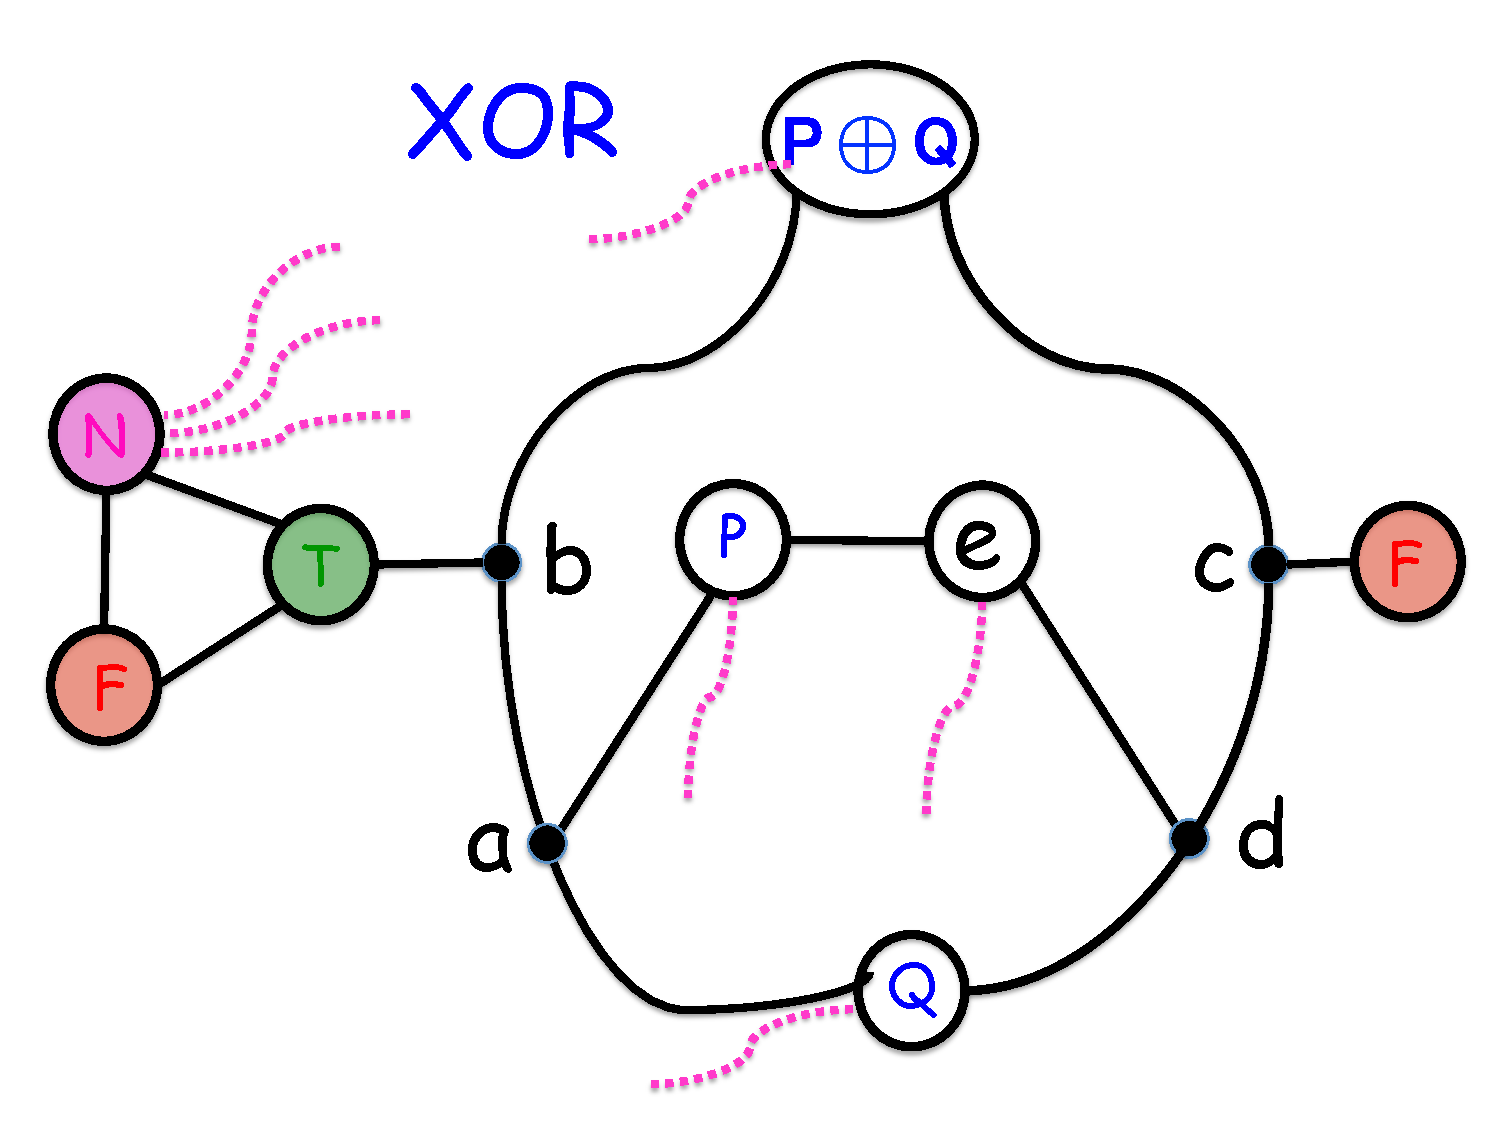
\includegraphics[width=4in]{3color-XOR}
\caption{A 3-color $\QXOR$-gate}
\label{fig:3color-XOR}
\end{figure}

%%%%%%%%%%%%%%%%%%%%%%%%%%%%%%%%%%%%%%%%%%%%%%%%%%%%%%%%%%%%%%%%%%%%%
% Problem ends here
%%%%%%%%%%%%%%%%%%%%%%%%%%%%%%%%%%%%%%%%%%%%%%%%%%%%%%%%%%%%%%%%%%%%%

\endinput
